

%仍需其他人审阅，我搞不懂教务处整的一堆奇奇怪怪的东西

\chapter{分班与专业}

\section{分班}

\subsection{班级组成}

中国科学技术大学本科阶段主要包括三类培养序列：强基班、英才班和普通班。

学校具备强基计划招收本科生的资格，并按照相应方案进行培养。。同时，科大也是“基础学科拔尖学生培养计划 2.0”的参与高校之一，生命科学学院设有贝时璋生命科技英才班，实行准入与准出制度，并根据学业表现进行动态管理。

需要特别说明的是：

\begin{itemize}
  \item \textbf{强基班与普通班}是\emph{招生阶段}的概念；
  \item \textbf{英才班}则是\emph{入学后}的培养概念；
  \item 英才班的生源来自\textbf{强基班与普通班}。
\end{itemize}

因此，可以将强基班理解为“具有特殊政策的普通班”，而英才班则是一个在入学后通过选拔形成的培养序列。

\begin{figure}[H]
    \centering
    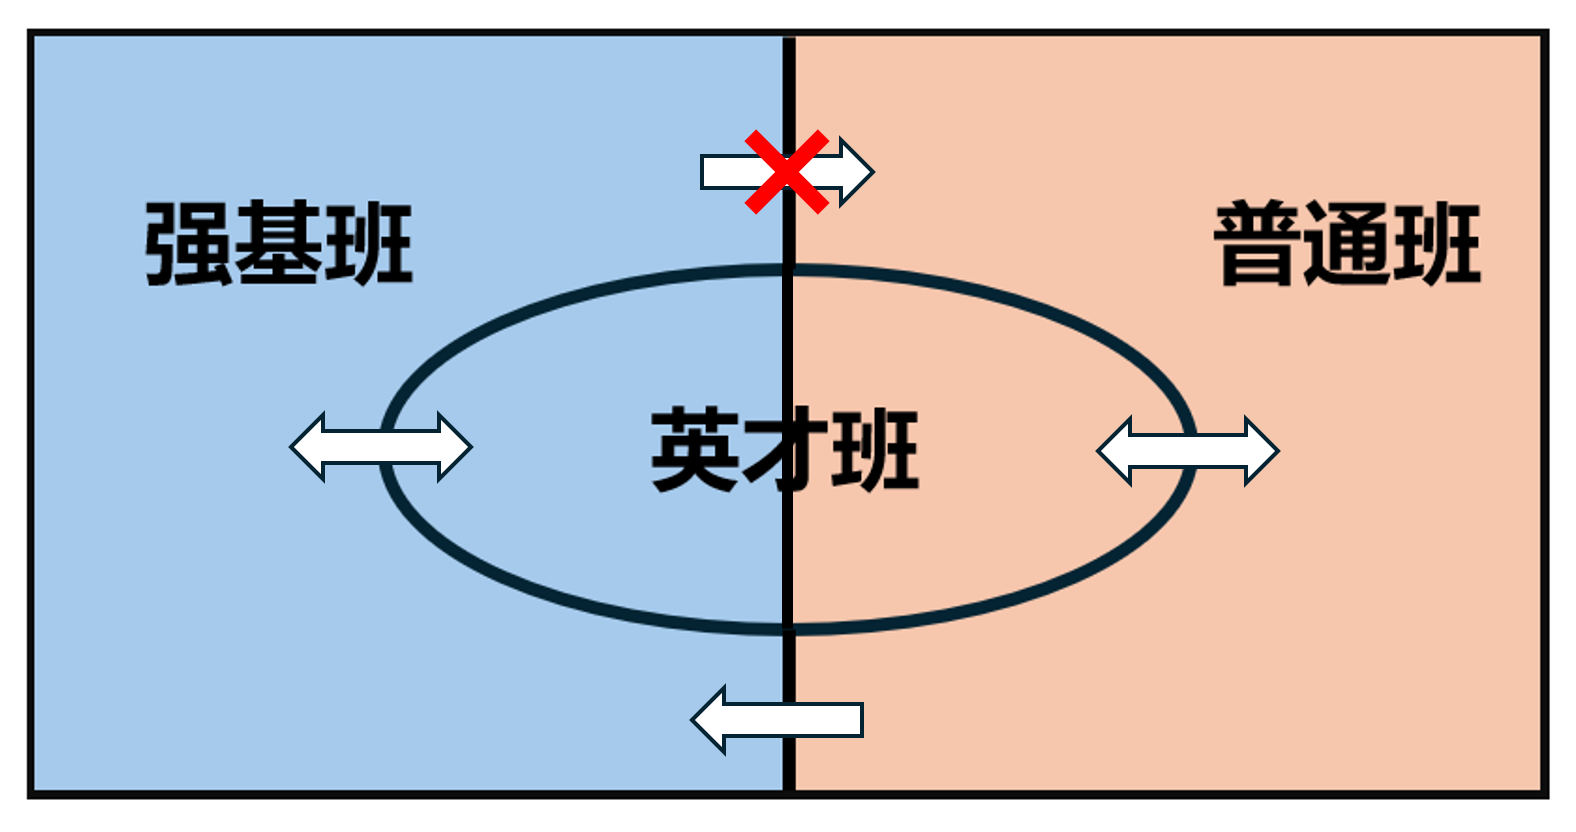
\includegraphics[width=0.5\textwidth]{image/分班与专业/分班veen.png}
    \caption{分班类型示意：英才班的生源来自强基班与普通班}
\end{figure}

\subsection{英才班与强基班的相关福利}

以 2022 级为例，各培养序列的主要“福利”情况如下（具体以当年政策为准）：

\textbf{英才班（2022 级）}
主要包括：
\begin{itemize}
  \item 免除学费的助学金；
  \item 必修的生物物理所与生化所实习（英才班培养方案必须）。实际每次实习时间约为 3 天，偶尔会和夏令营营员一起参加活动。
  \item 数量多但是实际教学收益有限且给分普遍偏低的课程。
\end{itemize}

\textbf{强基班（2022 级）}
主要包括：
\begin{itemize}
  \item 免除学费的助学金名额；
  \item 相对较低的本校保研分数线（\textbf{仅限本校}）。
\end{itemize}

需要注意的是：
\begin{itemize}
  \item 英才班与强基班的助学金名额比例均不高，且\textbf{二者互不占用}；
  \item 实习名额通常多于英才班名额，超出部分一般通过抽签决定，性质上更接近一次“免费参访”。
\end{itemize}

\textbf{不同转入情形的影响}

\begin{itemize}
  \item \textbf{强基班转入英才班：}  
  可以同时参与英才班以及强基班助学金竞争；需修读英才班课程；实习由“可能”变为“必定参加”。
  
  \item \textbf{普通班转入英才班：}  
  可参与英才班助学金评定；实习由概率事件变为确定事件；同时需承担英才班课程体系带来的学业压力。
  
  \item \textbf{普通班转入强基班：}  
  无法退出强基班（存疑，需要确认！）；保研仅限本校；可参与强基班助学金评定。该选择通常更适合绩点处于保研边缘、以稳定保研资格为主要目标的同学。
  
  \item \textbf{从英才班退出：}  
  由于培养方案差异，\textbf{存在补修课程的风险}。曾有同学在大二退出英才班，大四因需补修普通生物学实验课程而影响校外实习安排。具体要求以教秘解释为准，实际操作中存在一定不确定性。
  %找秦宇曈确认！！！！
\end{itemize}

综上所述：
\begin{itemize}
  \item 若不特别看重实习经历，\textbf{强基班并无明显必要转入英才班}；
  \item 若更关注经济支持，普通班转入英才班可视为\textbf{以 GPA 压力换取经济补助}；
  \item 若处于普通班保研边缘，转入强基班可以\textbf{降低本校保研风险}（但并非完全消除！）。
\end{itemize}

\subsection{培养方案与毕业条件}

\begin{figure}[H]
    \centering
    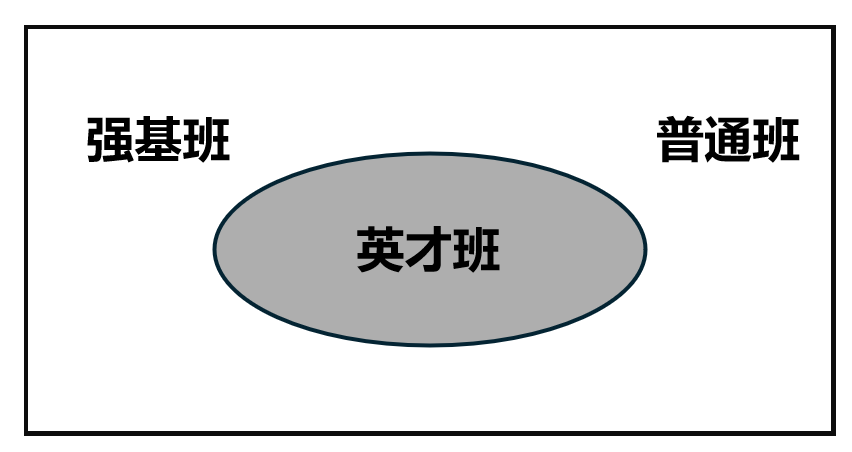
\includegraphics[width=0.5\textwidth]{image/分班与专业/培养方案veen.png}
    \caption{培养方案对比：普通班与强基班基本一致，英才班存在额外要求}
\end{figure}

各年级培养方案存在差异，请务必以\textbf{当年教秘发布信息}为准。总体来看，培养方案差异主要体现在\textbf{英才班与非英才班之间}，而非普通班与强基班之间。

以往情况显示，英才班在不修读部分给分较高的基础课程（如普通生物学、微生物学）的同时，需要额外修读生命科学前沿、生物医学论文写作等课程。虽然英才班课程在形式上不设优秀率限制，但这并不等同于实际评分宽松，且由于生源高度集中，\textbf{内卷现象较为明显}。

\section{专业选择}

\subsection{专业与保研要求}

生命科学学院本科阶段主要设有两个专业：\textbf{生物科学}与\textbf{生物技术}。

以 2026 Fall 为例，两专业主要差异体现在：
\begin{itemize}
  \item 专业选修课程（11.5 学分）设置不同；
  \item 保研必修课程要求有所差异。
\end{itemize}

生物科学通常是每年选择人数最多的专业，2026 Fall 约占 70\%，且排名靠前的同学多集中于该专业。若未来规划以\textbf{出国深造}为主，则可不必过度考虑保研必修课程的差异；在此情况下，由于竞争相对较小，选择生物技术专业有时更有利于获得较高排名。

需要指出的是，这一优势本质上来源于\textbf{信息差}，并非制度设计本身。一旦该情况被普遍认知，其有效性可能迅速下降，具体仍需以当年实际情况为准。

\begin{minipage}{0.44\textwidth}
  \centering
  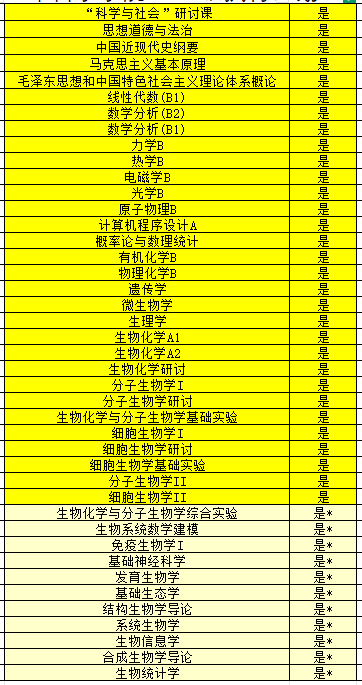
\includegraphics[width=0.88\textwidth]{image/分班与专业/生物科学.png}
\end{minipage}
\hspace{1em}
\begin{minipage}{0.45\textwidth}
  \centering
  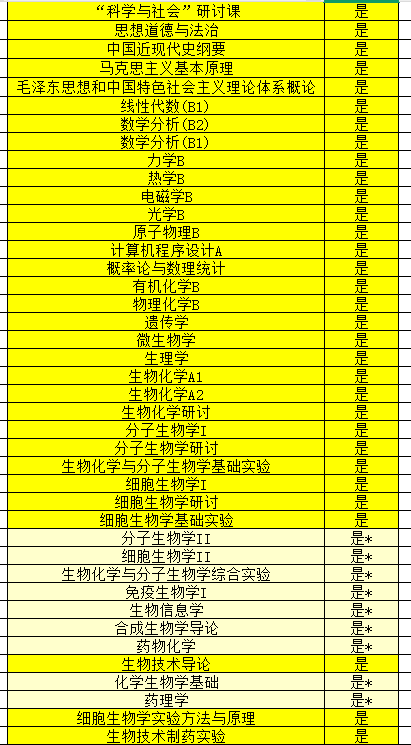
\includegraphics[width=0.9\textwidth]{image/分班与专业/生物技术类.png}
\end{minipage}

左图与右图分别为 2025 Fall 生物科学与生物技术专业的保研必修课程示意。

\begin{remark}
\textbf{以上保研必修课程信息基于 2025 Fall，具体要求请以当学年教秘发布内容为准。}  
2026 Fall 要求中，上图深黄色标注课程为必修课程，浅黄色标注课程需修满五门；英才班不需要修读微生物学。
\end{remark}
